\chapter{Additional Season-Level Simulations}
\label{appendix:season_level_simulations}

This appendix presents simulation graphics for seasons not detailed in the main text.
For each season, we show the championship probability evolution, relegation probability evolution, mid-season position probability heatmap, and end-of-season team strength estimates.
See Section~\ref{sec:club_applications} for detailed interpretation of these figures.

\section{2021 Season}
\label{sec:appendix_2021}

\begin{figure}[H]
    \centering
    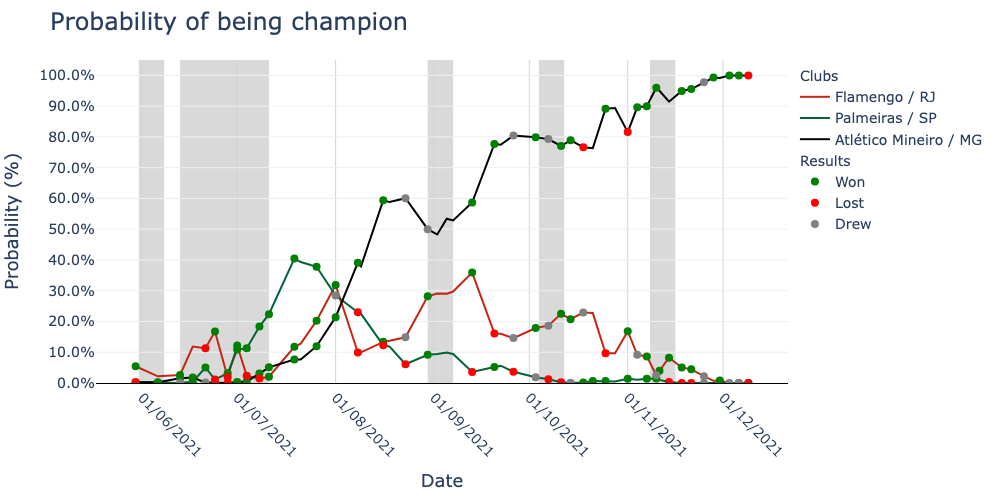
\includegraphics[width=\textwidth]{figures/2021_visualization_poisson_7_champ.png}
    \caption{\textbf{Championship probability evolution for the 2021 \textit{Brasileirão}}.}
    \label{fig:app_2021_champ}
\end{figure}

\begin{figure}[H]
    \centering
    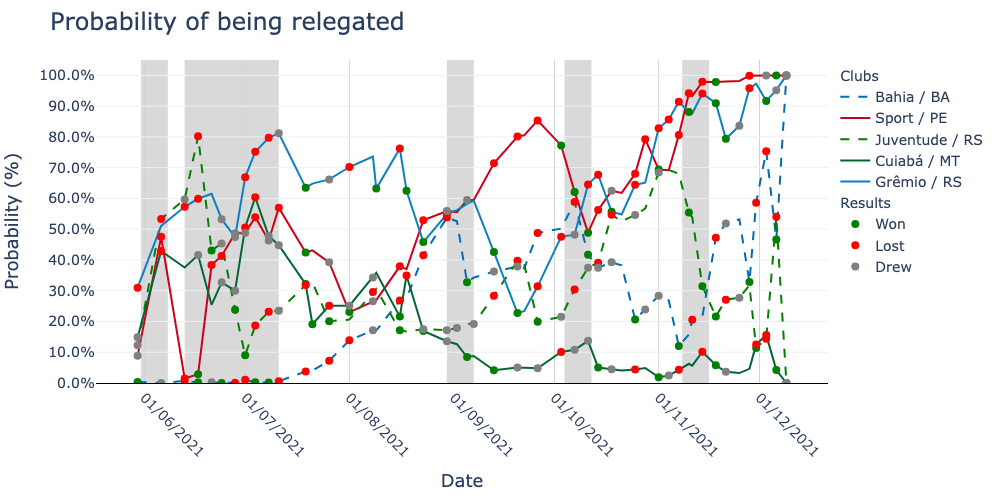
\includegraphics[width=\textwidth]{figures/2021_visualization_poisson_7_z4.png}
    \caption{\textbf{Relegation probability evolution for the 2021 \textit{Brasileirão}}.}
    \label{fig:app_2021_z4}
\end{figure}

\begin{figure}[H]
    \centering
    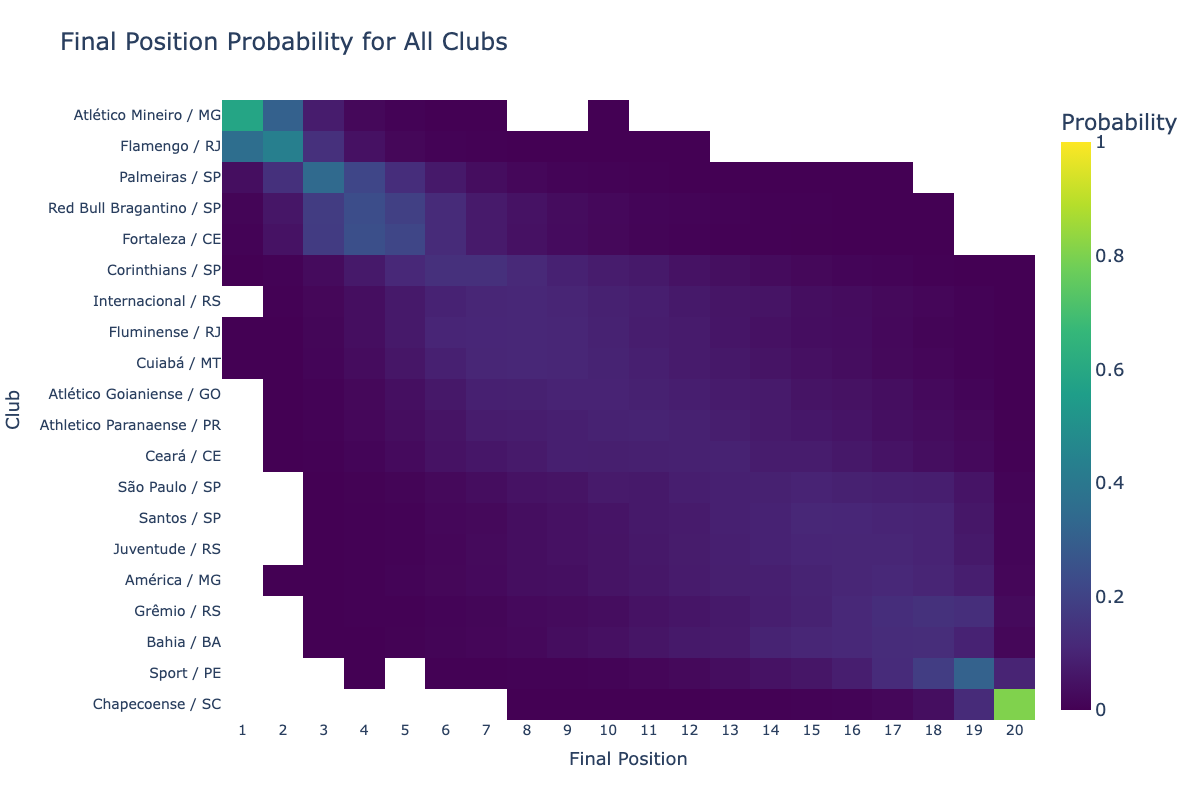
\includegraphics[width=\textwidth]{figures/2021_final_position_probs_all_clubs_193_poisson_7.png}
    \caption{\textbf{Final position probability distribution at mid-season 2021 (after 193 matches)}.}
    \label{fig:app_2021_positions}
\end{figure}

\begin{figure}[H]
    \centering
    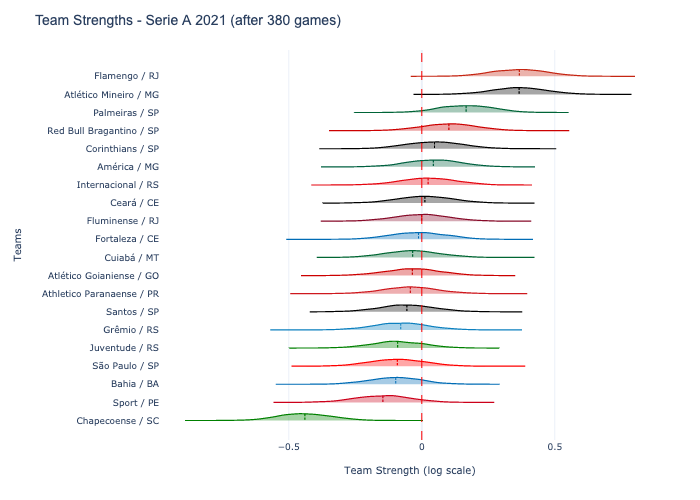
\includegraphics[width=0.9\textwidth]{figures/2021_team_strengths_violin.png}
    \caption{\textbf{Posterior distributions of team strengths for the 2021 \textit{Brasileirão}}.}
    \label{fig:app_2021_strengths}
\end{figure}

\section{2022 Season}
\label{sec:appendix_2022}

\begin{figure}[H]
    \centering
    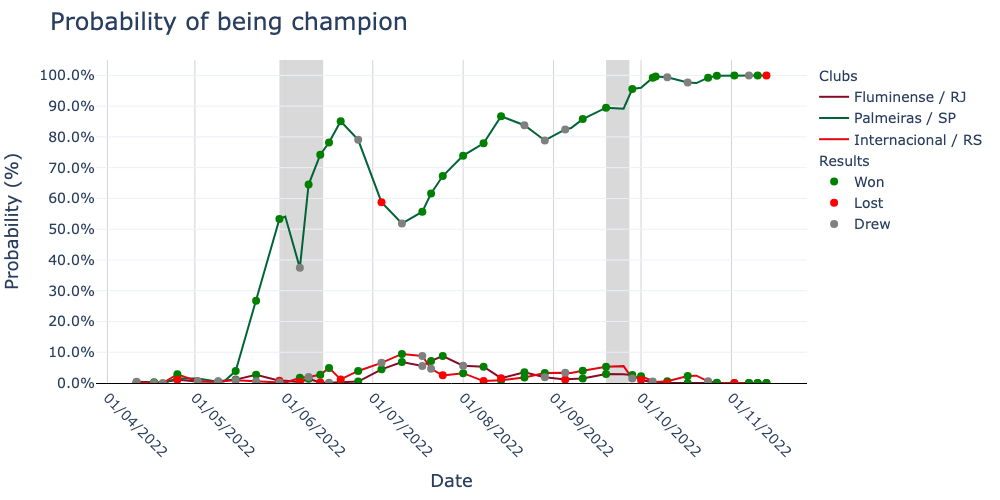
\includegraphics[width=\textwidth]{figures/2022_visualization_poisson_7_champ.png}
    \caption{\textbf{Championship probability evolution for the 2022 \textit{Brasileirão}}.}
    \label{fig:app_2022_champ}
\end{figure}

\begin{figure}[H]
    \centering
    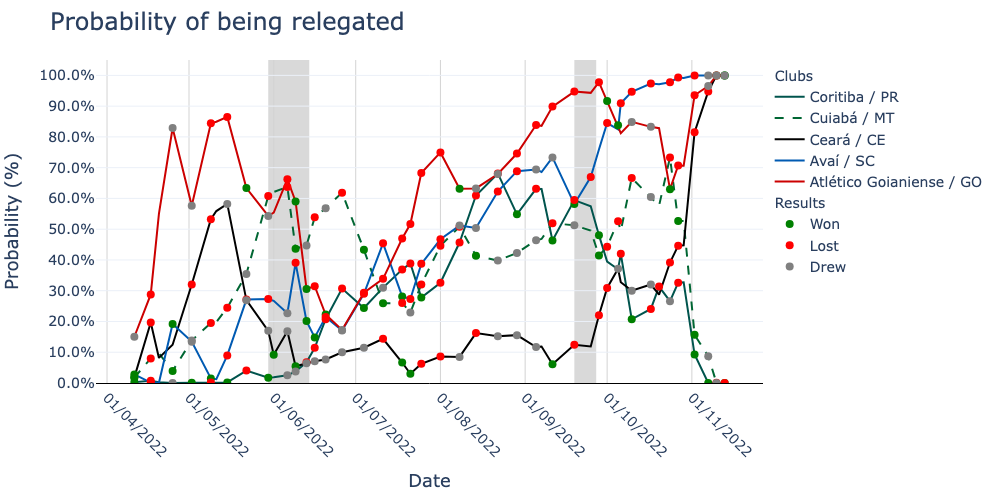
\includegraphics[width=\textwidth]{figures/2022_visualization_poisson_7_z4.png}
    \caption{\textbf{Relegation probability evolution for the 2022 \textit{Brasileirão}}.}
    \label{fig:app_2022_z4}
\end{figure}

\begin{figure}[H]
    \centering
    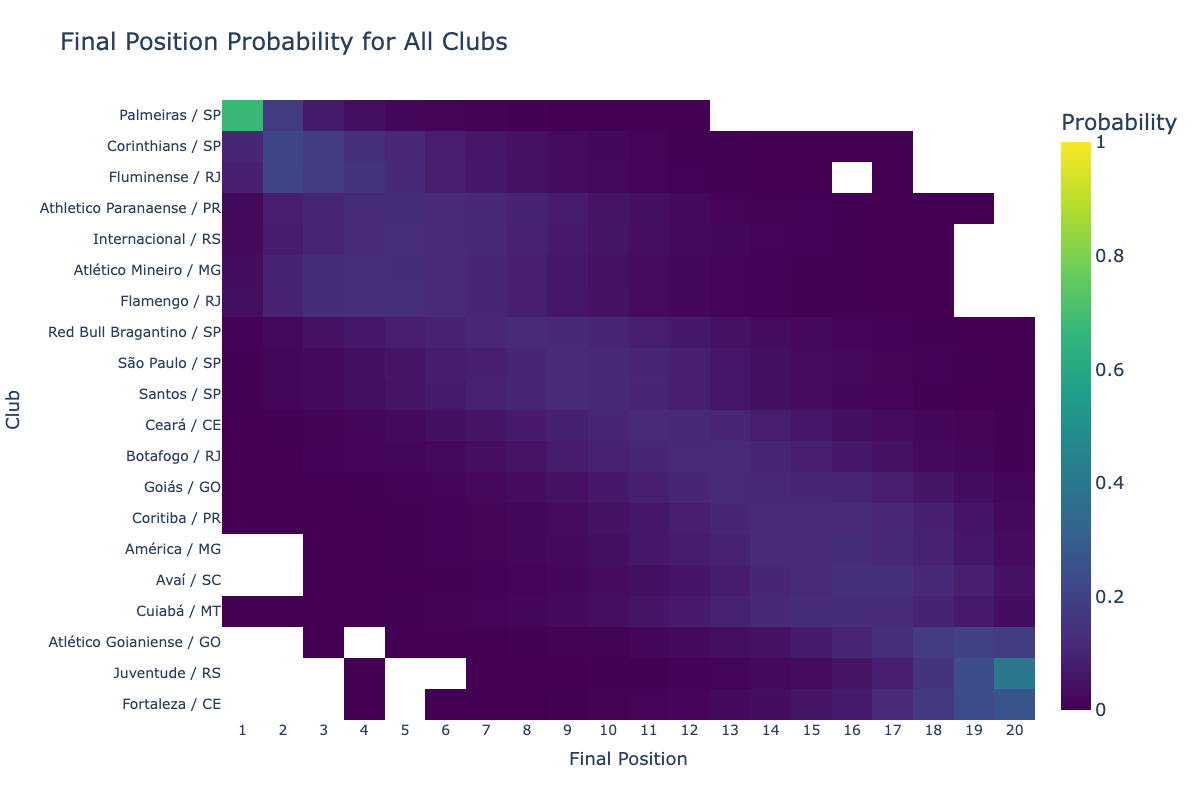
\includegraphics[width=\textwidth]{figures/2022_final_position_probs_all_clubs_190_poisson_7.png}
    \caption{\textbf{Final position probability distribution at mid-season 2022 (after 190 matches)}.}
    \label{fig:app_2022_positions}
\end{figure}

\begin{figure}[H]
    \centering
    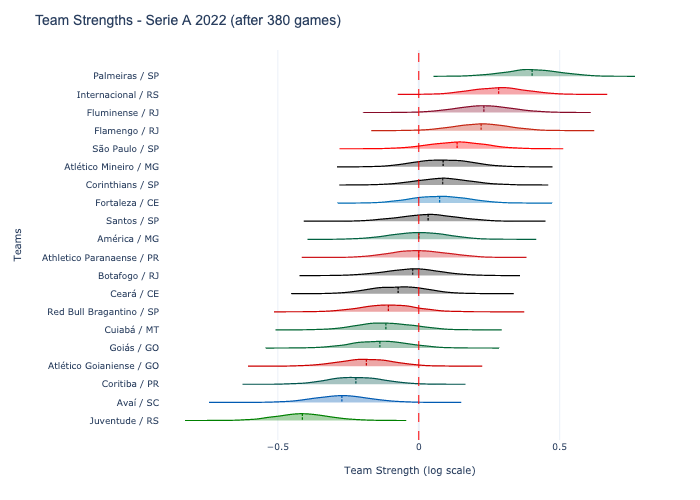
\includegraphics[width=0.9\textwidth]{figures/2022_team_strengths_violin.png}
    \caption{\textbf{Posterior distributions of team strengths for the 2022 \textit{Brasileirão}}.}
    \label{fig:app_2022_strengths}
\end{figure}

\section{2024 Season}
\label{sec:appendix_2024}

\begin{figure}[H]
    \centering
    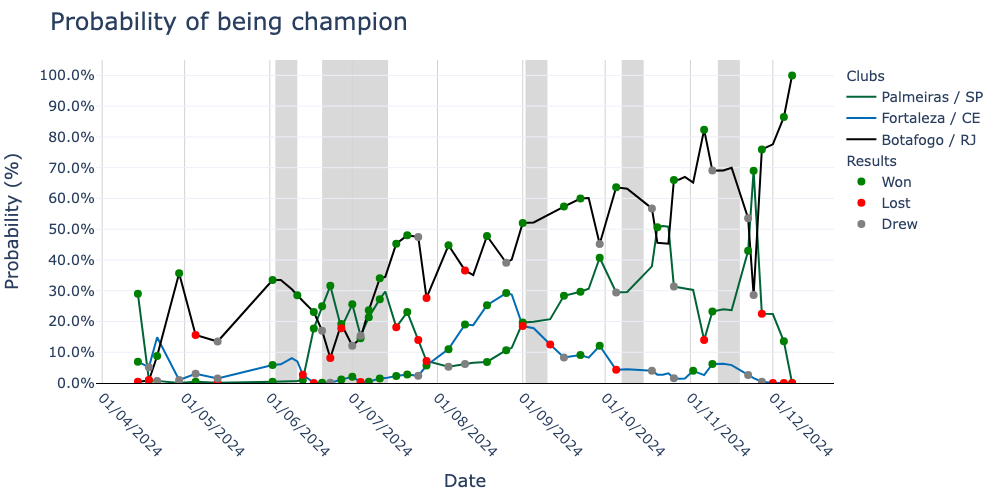
\includegraphics[width=\textwidth]{figures/2024_visualization_poisson_7_champ.png}
    \caption{\textbf{Championship probability evolution for the 2024 \textit{Brasileirão}}.}
    \label{fig:app_2024_champ}
\end{figure}

\begin{figure}[H]
    \centering
    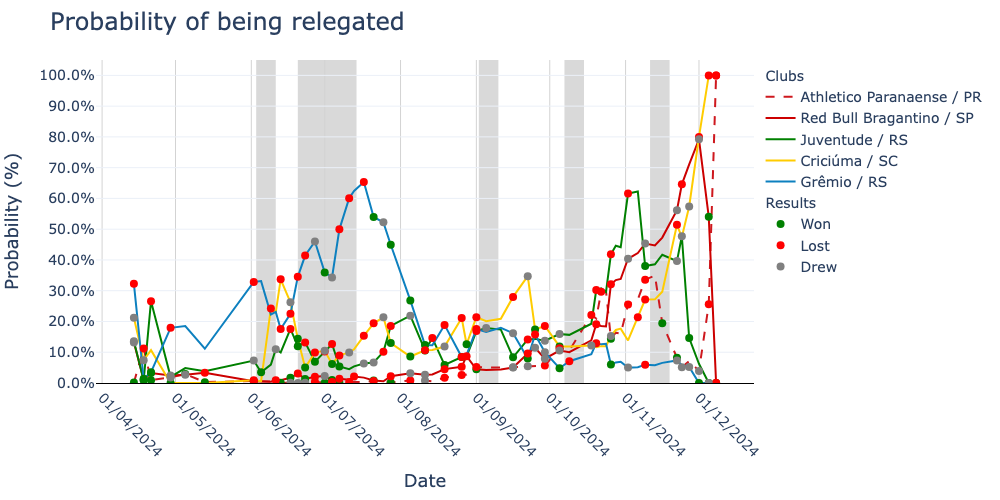
\includegraphics[width=\textwidth]{figures/2024_visualization_poisson_7_z4.png}
    \caption{\textbf{Relegation probability evolution for the 2024 \textit{Brasileirão}}.}
    \label{fig:app_2024_z4}
\end{figure}

\begin{figure}[H]
    \centering
    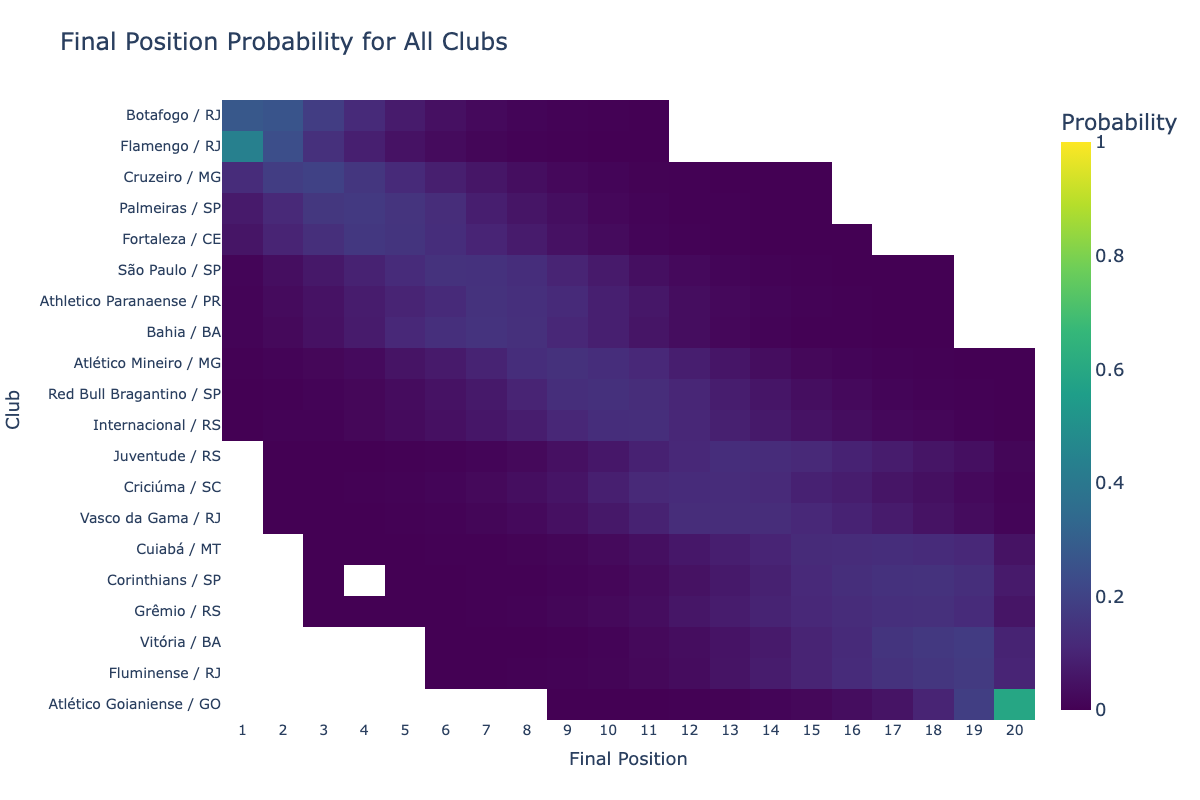
\includegraphics[width=\textwidth]{figures/2024_final_position_probs_all_clubs_188_poisson_7.png}
    \caption{\textbf{Final position probability distribution at mid-season 2024 (after 188 matches)}.}
    \label{fig:app_2024_positions}
\end{figure}

\begin{figure}[H]
    \centering
    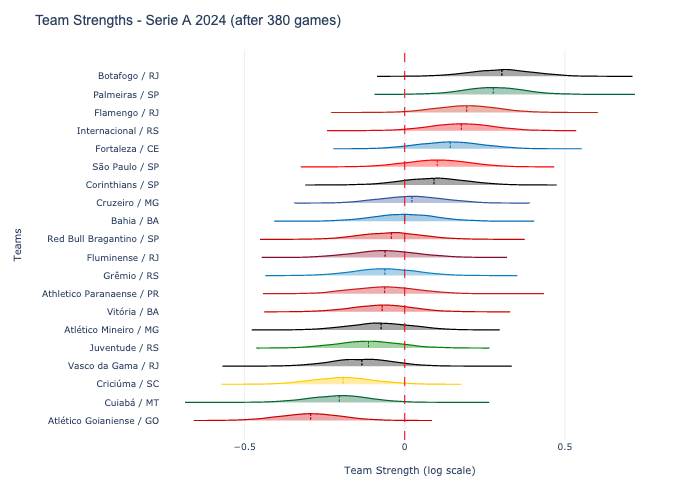
\includegraphics[width=0.9\textwidth]{figures/2024_team_strengths_violin.png}
    \caption{\textbf{Posterior distributions of team strengths for the 2024 \textit{Brasileirão}}.}
    \label{fig:app_2024_strengths}
\end{figure}
